%\externaldocument[-f]{c2_foundations}
\chapter{Methodology}
\label{chap:3}

This chapter presents the methodology used in this thesis. First, it is explained how different frameworks, which were introduced in \cref{chap:2}, are put into use. Then, the algorithms used in data generation and inference are given in detail. The results from these experiments are presented in the succeeding chapter.

\section{The Model}
\begin{wrapfigure}{R}{0.3\textwidth}
	\centering
	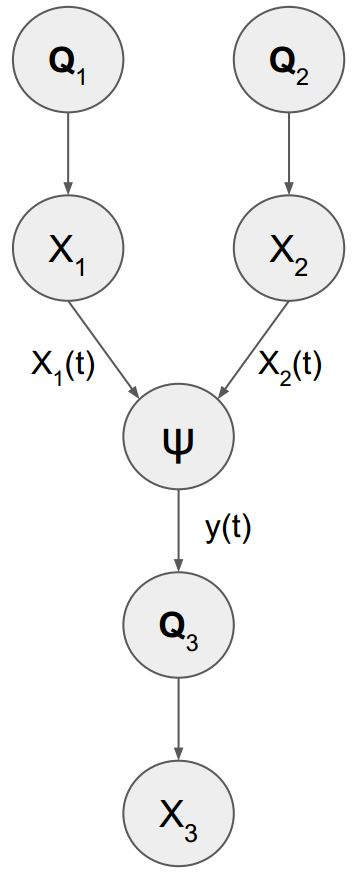
\includegraphics[width=0.6\linewidth]{figures/h_model}
	\caption{Hierarchical model.}
	\label{fig:h_model}
\end{wrapfigure} 
A detailed graphical model explored in this thesis is given in the \cref{fig:h_model}. This model presents an intersection of continuous-time Bayesian network and partially observable Markov decision process frameworks. 
\begin{itemize}
	\item The transition models of the nodes $ X_1, X_2$ and $ X_3 $, and the dependencies between them are modelled as CTBN.
	\item The interaction of agent node $ X_3 $ and its environment is modelled as POMDP.
\end{itemize}

\subsection{CTBN Model}
\label{sec:exp_ctbn_model}
The transition models of the nodes and the dependencies between them are modelled as continuous-time Bayesian network (CTBN), denoted by S with graph $ \mathcal{G} = \left( \mathcal{V}, \mathcal{E}\right) $, where $ \mathcal{V} = \left\lbrace X_1, X_2, X_3 \right\rbrace $ and $ \mathcal{E} = \left\lbrace (X_1, X_3), (X_2, X_3)\right\rbrace  $. The network S represents a stohastic process over a structured factorising state space $ \mathcal{S} = \rchi_1 \times \rchi_2 \times \rchi_3 $.\\
The parent nodes $X_{1}$ and $ X_{2} $ emit their states as messages. The dynamics  of these nodes are modelled as independent homogeneous continuous-time Markov processes $X_{i}(t)$, with binary-valued states $ \rchi_{i} = \left\lbrace 0, 1 \right\rbrace  $ for $ i \in \left\lbrace 1,2 \right\rbrace $. These processes are defined by transition intensity matrices $ \textbf{Q}_{i} $, which are assumed to be Gamma distributed with shape and rate parameters $ \symbf{\alpha} = [\alpha_0, \alpha_1] $ and $ \symbf{\beta} = [\beta_0, \beta_1] $, respectively, and are in the following forms.
\begin{align}
\textbf{Q}_i &= 
\begin{bmatrix}
-q^i_{0} & q^i_{0} \\
q^i_{1} &  -q^i_{1}
\end{bmatrix}
\label{eq:Q_parents}\\
\textbf{Q}_{i} &\sim \mathrm{Gam}(\symbf{\alpha}^i, \symbf{\beta}^i)\ \ for\ i \in \left\lbrace 1,2\right\rbrace \label{eq:gamma_priors}
\end{align}
It should be noted that in \autoref{eq:Q_parents}, the suffixes are simplified using the fact that $ q_{i} = \sum_{i \neq j} q_{i,j}$.\\
The agent  $ X_{3} $ is modelled as inhomogenouos continuous-time Markov process with binary states $ \rchi_{3} = \left\lbrace 0, 1 \right\rbrace  $ and set of actions $ a \in \left\lbrace a_0, a_1\right\rbrace  $, and set of transition intensity matrices which contains one matrix corresponding to each action, $ \textbf{\textit{Q}}_{3 \mid a} = \left\lbrace \textbf{Q}_{3\mid a_{0}}, \textbf{Q}_{3\mid a_{1}} \right\rbrace $.\\
%\begin{equation}
%\textbf{Q}_{a_k} \sim \mathrm{Gam}(\alpha_{a_k}, \beta_{a_k})
%\end{equation}
The dependencies are represented by set of parents for each node $ U_{n} = \mathrm{Par}_{\mathcal{G}}(X_n) $ and for the model shown in \cref{fig:h_model} can be written as follows:
\begin{align*}
U_{1}, U_{2} & = \emptyset \\
U_{3} & = \left\lbrace X_1, X_2 \right\rbrace 
\end{align*}
In order to have a compact representation of parent messages, a subsystem of S consisting of only the parent nodes, $ X_1 $ and $ X_2 $ can be considered as a single system. These two processes can be represented as a \textit{joint} process, $ X_P $, with factorising state space $ \rchi_{P} = \rchi_1 \times \rchi_2  $. The transition intensity matrix of the new joint system, $ \textbf{Q}_P $ is obtained by amalgamation operation, denoted by *, between $ \textbf{Q}_{1} $ and  $ \textbf{Q}_{2} $ (see \cref{ap:amalgamation}) \cite{Nodelman1995}.
\begin{equation}
\textbf{Q}_P = \textbf{Q}_{1} * \textbf{Q}_{2}
\end{equation}

\subsection{POMDP Model}
\label{sec:exp_pomdp_model}
In a conventional POMDP scenario, there are two problems to be addressed, one is belief state update and the other is policy optimization. As mentioned in \cref{sec:belief_POMDP}, in the problem at hand, the policy of agent $ X_3 $ is assumed to be optimal and given. Thus, the POMDP model of the agent only consists of belief state update. A detailed view of the agents interaction with its environment from POMDP framework perspective is given in the \cref{fig:POMDP_pers}. \\
\begin{figure}[H]
	\begin{center}
		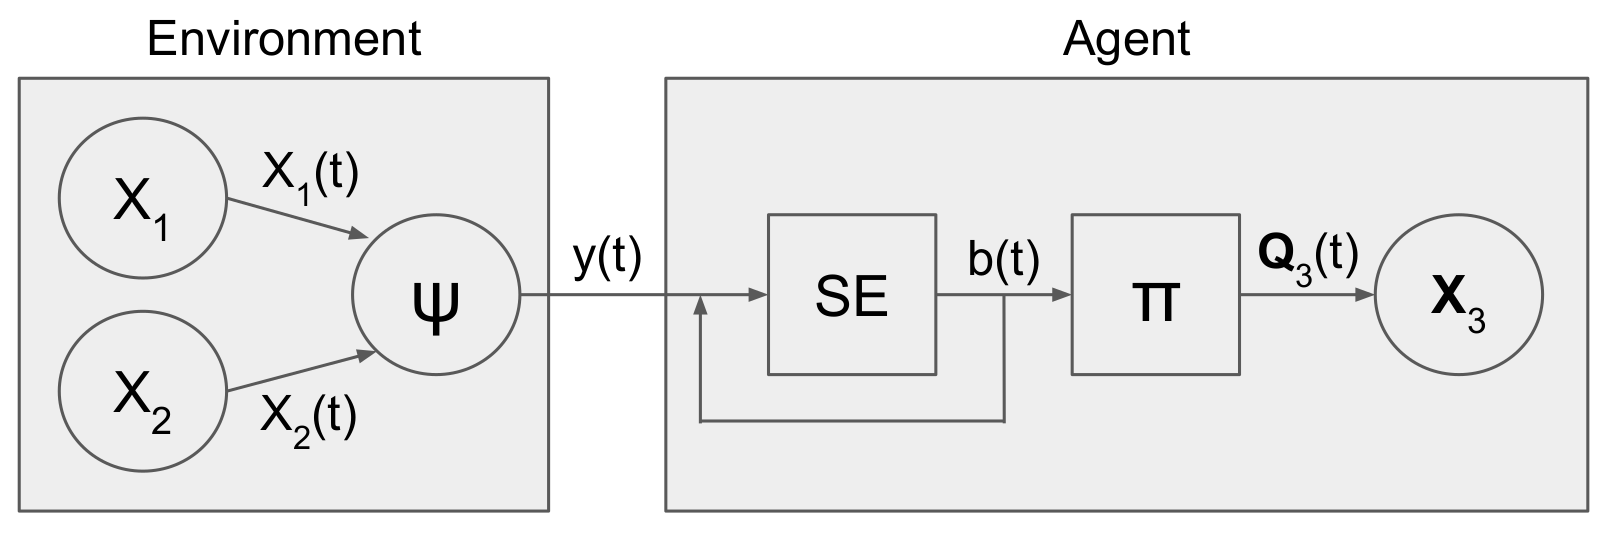
\includegraphics[width=.75\textwidth]{figures/POMDP_graph}
		\caption{Closer look to agent-environment interaction from the perspective of POMDP framework.}
		\label{fig:POMDP_pers}
	\end{center}
\end{figure}
It should be noted that, the interaction in \cref{fig:POMDP_pers} is only one-sided, the state or action of the agent does not affect the environment.
\subsubsection{Observation Model}
\label{sec:observ_model}
The messages sent by the parent nodes are translated by the observation model. The agent node $ X_3 $ does not have a direct access to the messages, but observes a translation of them. The observation is denoted by $ y(t) = y_t $ such that $ y_t \in \mathcal{Y} $ where $ \mathcal{Y} $ is the observation space. The observation model defines a probability distribution over the observation for each combination of parent messages.
\begin{equation}
\psi(x_1, x_2) = p(y(t) \mid X_{1}(t)=x_1, X_{2}(t)=x_2)
\label{eq:obs_model_two_system}
\end{equation}
where $ x_1 \in \rchi_1 $ and $ x_2 \in \rchi_2 $. As explained in \cref{sec:exp_ctbn_model}, using the joint process $ X_P $ for the sake of conciseness, \autoref{eq:obs_model_two_system} can be written as
\begin{equation}
\psi(x_P) = p(y(t) \mid X_P(t)=x_P)
\label{eq:obs_model_p}
\end{equation}
where $ x_P \in \rchi_P $. \\
$ \psi(x_P) $ is defined as deterministic categorical distribution over the observation space $ \mathcal{Y} $. For each state $ x_P $, there is one possible observation $ y_i \in \mathcal{Y} $, such that \begin{equation}
p(y_i \mid x_P) = 1 \;\wedge \;p(y_j \mid x_P) = 0 \quad \forall j \neq i .
\label{eq:det_cat_dist}
\end{equation} 
$ \psi $ denotes the matrix with rows $ \left\lbrace \psi(x_P)\right\rbrace_{x_P \in \rchi_P} $.
\subsubsection{Belief State}
The belief state provides a summary over agents past experiences and allows the agent to take its own uncertainty into account. The belief state is formed by the \textit{state estimator} (labelled as \textit{SE} in \cref{fig:POMDP_pers}) over the parent states, denoted by $  b(x_P; t) $. 
\begin{equation}
b(x_P; t) = \operatorname{Pr}( X_P(t) = x_P \mid y_{1}, ..., y_{t})
\end{equation}
\paragraph*{Exact Belief State Update}
\label{par:bs_exact}
As discussed in \cref{sec:filtering_CTMC}, given the transition intensity matrices of parent nodes, $ \textbf{Q}_1 $ and $ \textbf{Q}_2 $, the continuous-time belief state update poses a filtering problem for CTMPs. This problem can be formulated according to the joint process of parents.
\begin{equation}
b(x_P; t) = \operatorname{Pr}( X_P(t) = x_{p} \mid y_{1}, ..., y_{t})
\end{equation}
Consider discrete-time observations from this process, denoted by $ y_{1}=y(t_{1}), ..., y_{l}=y(t_{l}) $ and time-dependent belief state $ b(t) $ as a row vector with $ \left\lbrace b(x_P;t)\right\rbrace_{x_P \in \rchi_P} $. Following \autoref{eq:b_cont} and \autoref{eq:b_jump}, the belief state update is evaluated as
\begin{equation}
b(t) = b(0) \exp(t\textbf{Q}_P)
\end{equation}
with the initial condition $ b(0) $.
The update at discrete times of observation $ y_{t} $ is
\begin{align}
b(x_P; t_{l}) &= Z_{l}^{-1}\ {p(y_{l} \mid X_P(t_{l})=x_P)}\ {b(x_P; t_{l}^{-})} \\ & = Z_{l}^{-1}\ \psi(x_P) \ {b(x_P; t_{l}^{-})}
\label{eq:bs_exact}
\end{align}
where $ Z_{l} = \sum_{x_P\in \rchi_P} \psi(x_P)\ b(x_P; t_{l}^{-}) $ is the normalization factor.
\paragraph*{Belief State Update Using Marginalized Particle Filter}
\label{par:bs_partFilt}
The assumption that full information of parent dynamics being available is unrealistic. In an environment as described above, the agent is more likely not to have access to the parameters $ \textbf{Q}_1 $ and $ \textbf{Q}_2 $, may rather have some prior beliefs over them. Moreover, when the state estimator utilizes exact update method, these parameters are assumed to be available for the inference as well. Thus, in order to simulate a more realistic model and be able to marginalize out these parameters from inference problem, the joint parent process $ X_P $ is replaced with its marginalized counterpart. Using the Gamma-priors over $ \textbf{Q}_1 $ and $ \textbf{Q}_2 $ (\autoref{eq:gamma_priors}) and sufficient statistics over the particle history, the particles are drawn from this marginalized process as explained in \cref{sec:marg_ctbn}. With every new observation, the particles are propogated through the marginal process, while the sufficient statistics are updated and the parameters are re-estimated after each particle using the \autoref{eq:estimated_Q}. The belief state then obtained as the distribution of states over the particles,
\begin{equation}
b(x_P; t) = \frac{1}{N} \sum_{i=1}^{N} \delta_{k_i(t), x_P}
\end{equation}
where $ N $ is the number of particles, $ k_i \in \textbf{k} $ is the set of particles, and $\delta$ is the Kronecker delta.

\begin{algorithm}[H]
	\SetKwInOut{KwIn}{Input}
	\SetKwInOut{KwOut}{Output}
	\KwIn{Observation $ y_{l} $ at time $ t_{l} $, set of particles $\textbf{k}^{l-1} $, estimated $ \hat{Q} $}
	\KwOut{New set of particles $ \textbf{k}^{l} $, $ \textbf{b}^{[t_{l-1}, t_{l}]} $}
	
	\vspace{+4pt}
	\begin{algorithmic}[1]
		\FOR{$k_{m} \in \textbf{k}^{l-1}$}
		\STATE {$k_{m} = \left\lbrace x_{m}, \hat{Q}\right\rbrace \leftarrow Propagate\ particle\ through\ marginal\ process\ from\ t_{l-1}\ to\ t_{l}$ }\\
		
		\STATE {$\hat{Q} \leftarrow sufficient\ statistics\ added\ from\  k_{m}[t_{l-1}, t_{l}]$} \\
		\tcp*[h] {observation likelihood assigned as particle weight}
		\STATE{$w_{m} \leftarrow p(y_{l} \mid X_P(t_{l})=x_{m}) $} \label{lst:weight_update}
		\ENDFOR \\
		\tcp*[h]{belief state from $ t_{l-1} $ to $ t_{l} $}
		\STATE{$ \textbf{b}^{[t_{l-1}, t_{l}]} \leftarrow \left\lbrace \frac{1}{N} \sum_{i=1}^{N} \delta_{k_i^{[t_{l-1}, t_{l}]} , x_P}\right\rbrace_{x_P \in \rchi_P} $}\\
		\tcp*[h]{normalize weights}
		\STATE{$ w_{m} \leftarrow \frac{w_{m}}{\sum_{m} w_{m}}$   }\\
		\tcp*[h]{  resample particles}
		\FOR{$ k_{m} \in \textbf{k}^{l} $} 
		\STATE{$ k_{m} \leftarrow Sample\ from\ \textbf{k}^{l}\ with\ probabilities\ w_{m}\ with\ replacement$}
		\ENDFOR 
	\end{algorithmic}
	\caption{Marginal particle filter for belief state update \cite{Studer2016}}
	\label{alg:part_filter}
\end{algorithm}
In \cref{alg:part_filter}, the weight update for the particles is performed on line \autoref{lst:weight_update}, based on the observation model. Given the deterministic nature of the observation model as described in \autoref{eq:det_cat_dist}, in rare cases where the observation $ y_k $ stems from an unlikely transition of parent nodes, the particles fail to simulate this transition and all of them get rejected. One possible solution to this problem would be increasing the number of particle to increase the probability of sampling unlikely transitions. However, in practice, this solution is not feasible due to computational cost. Instead, the degeneration of the particle filter is dealt with by assigning uniform probabilities to the particles, effectively ignoring the unlikely transitions. The situation is illustrated by examples from simulation in \cref{sec:simulation}.

\subsubsection{Optimal Policy}
The optimal policy is defined using a polynomial function of belief state.
\begin{equation}
\pi(b) = 
\begin{cases}
a_0 & \quad \text{if } \textbf{w}b^\intercal > 0.5 \\
a_1 & \quad \text{otherwise}
\end{cases}
\label{eq:policy}
\end{equation}
where \textbf{w} is a row vector of weights.\\
Given the optimal policy, $ \pi(b) $, the agent takes an action based on the belief state. In the setting described above, taking an action means to change its internal dynamics to the transition intensity matrix corresponding to that action.
\begin{align}
a(t) &= \pi(b(t))\\
\textbf{Q}_3(t) & = \begin{cases}
\textbf{Q}_{3\mid a_{0}} & \quad \text{if } a(t) = a_0 \\
\textbf{Q}_{3\mid a_{1}} & \quad \text{otherwise}
\end{cases}
\label{eq:Q_3_traj}
\end{align}

\section{Inference of Observation Model}
\label{sec:inf_setup}
Inference problem is considered for deterministic observation models, such that each state $ x_P \in \rchi_P $ can only be translated to one observation. Considering the number of states of parents and the observations, this results in a number of possible observation models. \\
Consider a trajectory in the dataset, denoted by $ S^{[0,T]} = \left\lbrace X_1^{[0,T]} , X_2^{[0,T]}, X_3^{[0,T]}\right\rbrace $. The set of parameters to the system, as introduced before, is written as $  \theta = \left\lbrace  \textbf{Q}_{1}, \textbf{Q}_{2}, \textit{\textbf{Q}}_3, \pi, \psi \right\rbrace $. Given the parent trajectories, $ X_1^{[0,T]} $ and $ X_2^{[0,T]} $, the belief state and the resulting $ \textbf{Q}_3 $ trajectory is computed for each observation model. Then the likelihood of $ S^{[0,T]} $ trajectory given the parameters $ \theta $ are compared for maximum likelihood estimation.
\begin{equation}
\hat{\psi} = \argmax_\psi p(S^{[0,T]} \mid \theta )
\label{eq:max_llh_est}
\end{equation}

\subsection{Likelihood Model}
 The likelihood of a sample trajectory $ S^{[0,T]} $ can be written as:
\begin{align}
p(S^{[0,T]} \mid \theta ) & = p(X_{1}^{[0, T]}, X_{2}^{[0, T]}, X_{3}^{[0, T]} \mid \textbf{Q}_{1}, \textbf{Q}_{2}, \textit{\textbf{Q}}_3, \pi, \psi) \nonumber\\
& = p(X_{3}^{[0, T]} \mid X_{1}^{[0, T]}, X_{2}^{[0, T]}, \textbf{Q}_{1}, \textbf{Q}_{2}, \textit{\textbf{Q}}_3, \pi, \psi) \ p(X_{1}^{[0, T]}\mid \textbf{Q}_{1}) \ p(X_{2}^{[0, T]}\mid \textbf{Q}_{2}) \nonumber\\ & = p(X_{3}^{[0, T]} \mid X_{1}^{[0, T]}, X_{2}^{[0, T]}, \textit{\textbf{Q}}_3, \pi, \psi) \ p(X_{1}^{[0, T]}\mid \textbf{Q}_{1}) \ p(X_{2}^{[0, T]}\mid \textbf{Q}_{2}) \nonumber\\ & = p(X_{3}^{[0, T]}\mid \textbf{Q}_{3}^{[0, T]}) \ p(X_{1}^{[0, T]}\mid \textbf{Q}_{1}) \ p(X_{2}^{[0, T]}\mid \textbf{Q}_{2}) 
\label{eq:system_llh}
\end{align}
As mentioned before, it is plausible to marginalize out the parameters $ \textbf{Q}_1 $ and $ \textbf{Q}_2 $, for a more realistic model and inference. Noting that in case the belief state is updated using filtering of CTMPs (See \cref{par:bs_exact}), $ \textbf{Q}_{3}^{[0, T]} $ becomes a deterministic function of all the parameters including $ \textbf{Q}_1 $ and $ \textbf{Q}_2 $, the marginalization cannot be carried out analytically on \autoref{eq:system_llh}. On the other hand, marginal particle filtering removes this dependency on $ \textbf{Q}_1 $ and $ \textbf{Q}_2 $ by using marginalized counterpart of CTMPs (See \cref{par:bs_partFilt}), leaving it straightforward to marginalize out the parameters on \autoref{eq:system_llh}.

Marginalizing the likelihood over $ Q_{1} $ and $ Q_{2} $:
\begin{align}
p(S^{[0,T]} \mid \pi, \psi ) & = 	\int \int p(S^{[0,T]} \mid \theta ) \ p(\textbf{Q}_{1}) \ p(\textbf{Q}_{2}) \ d\textbf{Q}_{1}d\textbf{Q}_{2} \nonumber\\ 
& = \int \int p(X_{3}^{[0, T]}\mid \textbf{Q}_{3}^{[0, T]}) \ p(X_{1}^{[0, T]}\mid \textbf{Q}_{1}) \ p(X_{2}^{[0, T]}\mid \textbf{Q}_{2}) \ p(\textbf{Q}_{1}) \ p(\textbf{Q}_{2})\ d\textbf{Q}_{1}d\textbf{Q}_{2} \nonumber\\ 
& = p(X_{3}^{[0, T]}\mid \textbf{Q}_{3}^{[0, T]}) \int  p(X_{1}^{[0, T]}\mid \textbf{Q}_{1}) \ p(\textbf{Q}_{1}) \ d\textbf{Q}_{1} \int p(X_{2}^{[0, T]}\mid \textbf{Q}_{2})\ p(\textbf{Q}_{2})\ d\textbf{Q}_{2}
\label{eq:Marg_llh}
\end{align}
Marginalized likelihood function for binary-valued homogenous CTMP is derived in \autoref{ap:marg_llh_ctmp}.

Plugging \autoref{eq:Marg_traj} in \autoref{eq:Marg_llh} for both $ X_{1} $ and $ X_{2} $:
\begin{align}
\begin{split}
p(S^{[0,T]} \mid \pi, \Phi ) = p(X_{3}^{[0, T]}\mid Q_{3}^{[0, T]}) \prod_{x_{1}\in{0,1}} \frac{\beta_{x_{1}}^{\alpha_{x_{1}}}}{\Gamma(\alpha_{x_{1}})} \ (T_{x_{1}}+\beta_{x_{1}})^{M_{x_{1}} + \alpha_{x_{1}}}\ \Gamma(M_{x_{1}} + \alpha_{x_{1}})  \\  \prod_{x_{2}\in{0,1}} \frac{\beta_{x_{2}}^{\alpha_{x_{2}}}}{\Gamma(\alpha_{x_{2}})} \ (T_{x_{2}}+\beta_{x_{2}})^{M_{x_{2}} + \alpha_{x_{2}}}\ \Gamma(M_{x_{2}} + \alpha_{x_{2}})
\label{eq:Marg_llh_final}
\end{split}
\end{align}
In order to avoid numerical unstability, the log-likelihood is preferred for the calculations instead of likelihood.
\subsection{Inference under Noisy Observation Model}
In order to assess the robustness of the inference, we added an error probability $ p_e $ to the observation model. As explained in \cref{sec:observ_model}, the observation model $ \psi(x_P) $ is assumed to be deterministic. This corresponds to a unique translation, denoted here by $ y_\text{true} $ of each parent state $ x_P $. In the case of noisy observation model, the resulting observation might differ from the correct translation $ y_\text{true} $ with probability $ p_e $, and the erroneous translation is drawn uniformly from the remaining observation space $ y_i \in \mathcal{Y} \backslash \left\lbrace y_\text{true}\right\rbrace $. This noisy observation model is denoted by $ \psi^{p_e} $ can be considered as a noisy communication channel with error probability $ p_e $. \begin{equation}
p(y_\text{true} \mid x_P) = 1-p_e \;\wedge \;p(y_j \mid x_P) = \frac{p_e}{|\mathcal{Y}|-1} \quad \forall y_j \neq y_\text{true}
\label{eq:noicy_obs_model}
\end{equation} 
For simulation, the noisy observation model is assumed to be available to the agent, which mainly affects the agent's belief state. For exact belief state update, the noisy observation model is employed in \autoref{eq:bs_exact}. In the case of particle filtering, the weights are assigned to the particle using the noisy model (see \cref{alg:part_filter}, line \autoref{lst:weight_update}). It is noteworthy that by doing so, the degeneration of particle filter as described in \cref{par:bs_partFilt} is prevented.

\section{Data Generation}
The dataset contains a number of trajectories drawn from CTBN S. Following the notation in \cref{chap:2}, K trajectories in time interval $ [0, T] $ are denoted by $ \xi_T = \left\lbrace S^{[0,T], 1}, S^{[0,T], 2}, ..., S^{[0,T], K} \right\rbrace  $, where $ S^{[0,T],k} = \left\lbrace X_1^{[0,T],k} , X_2^{[0,T],k}, X_3^{[0,T],k}\right\rbrace $ denotes a single trajectory for all nodes. Every trajectory comprises of state transitions in the interval, and the times of these transitions. 

\subsection{Sampling Algorithm}
In order to sample trajectories from CTBN, two sampling algortihms introduced in \cref{sec:sampling_alg} are combined. Gillespie algorithm is used to sample from the parent nodes, $ X_1 $ and $ X_2 $, while thinning algorithm is applied to overcome the challenges that come with conditional intensity matrix of the agent, $ X_3 $. It should be noted that \cref{alg:generative_ctbn} is applicable to any nodes in a CTBN, both homogenous and conditional MPs. However, since in this setting, the intensity matrix is conditioned on the belief state and the policy, instead of directly on the parent states, a more general algorithm suitable for inhomogenous MPs, thinning algorithm, is preferred. \cref{alg:sampling} describes the procedure to draw samples using marginal particle filtering. 

\begin{algorithm}[H]
	\SetKwInOut{KwIn}{Input}
	\SetKwInOut{KwOut}{Output}
	\SetKwInOut{Init}{Initialize}
	
	\KwIn{Gamma-prior parameters on parents' transition intensity matrices $ \alpha^1, \beta^1, \alpha^2, \beta^2 $\\
		Set of agent's transition intensity matrices $ \textbf{\textit{Q}}_3 $\\
		$ T_{max} $ to terminate simulation}
	\KwOut{Sample trajectory of the network}
	\Init{Sample $ \textbf{Q}_1 $ and $ \textbf{Q}_2 $ from their priors\\ 
		Initialize nodes uniformly $ X_{n}(0) = x_{i} \in \rchi_n$ \\
		Initialize particles uniformly $ p^i(0) = x_{p} \in \rchi_P$\\
		$ t=0 $}
	
	\begin{algorithmic}[1]
		\WHILE{$ t < T_{max} $}
		\STATE{Draw next transition for $ X_1 $ and $ X_2 $ ($ \tau_{parent}$, $ x_1 $ and $ x_2 $ using \cref{alg:generative_ctbn})}
		\STATE{$ t_{parent} \leftarrow t + \tau_{parent} $}	\tcp*[h]{transition time for parents} 
		\STATE{$ y_{t_{parent}} \sim \psi(x_1, x_2)$} \tcp*[h]{new observation at $ t_{parent} $}
		\STATE{Update particle filter and obtain $ \textbf{b}^{[t, t_{parent}]} $}
		\STATE{$ a^{[t, t_{parent}]} \leftarrow \pi(\textbf{b}^{[t, t_{parent}]}) $}
		\STATE{$ \textbf{Q}_3^{[t, t_{parent}]} \leftarrow \textbf{Q}_{3\mid a^{[t, t_{parent}]}} $}
		\STATE{$ t_{agent} \leftarrow t$}
		\WHILE{$ t_{agent} < t_{parent} $}
		\STATE{\text{the upper bound for intensity,} $ q_3^{*}$} \footnotemark
		\STATE{\text{transition time $ \tau_{agent} $ drawn by }  $ u \sim U(0, 1)$ \text{ and } $ \tau_{agent} = \frac{-ln(u)}{q_3^{*}} $}
		\STATE{$ t_{agent} \leftarrow t_{agent} + \tau_{agent} $}
		\STATE{\text{draw } $s \sim U(0, 1)$, \text{accept transition if} $ s \leq \frac{q_3(t_{agent})}{q_3^{*}}$}
		\ENDWHILE
		\STATE{$ t \leftarrow t_{parent} $}
		\ENDWHILE
	\end{algorithmic}
	\caption{Sampling trajectories with marginal particle filtering}
	\label{alg:sampling}
\end{algorithm}
\footnotetext{q is the transition intensity associated with the current state of the agent.}

%\begin{table}[!htb]
%	\begin{minipage}{.5\linewidth}
%		%		\centering
%		\begin{tabular}{c c}
%			\hline 
%			\textbf{Parameter} & \textbf{Value} \\ 
%			\hline 

%			\hline 
%		\end{tabular}
%		\caption{configuration}
%	\end{minipage}%
%	\begin{minipage}{.5\linewidth}
%		%		\centering
%		\begin{tabular}{c c c}
%			\hline 
%			\textbf{Parameter} & \textbf{Value} 
%			\hline 

%			\hline 
%		\end{tabular}
%		\caption{configurations}
%	\end{minipage} 
%\end{table}
